\documentclass[tikz,border=5pt]{standalone}
\usepackage{tikz}
\usetikzlibrary{arrows.meta,positioning,calc}
\definecolor{nebula}{HTML}{6366F1}
\definecolor{spark}{HTML}{14B8A6}
\definecolor{ink}{HTML}{334155}
\begin{document}
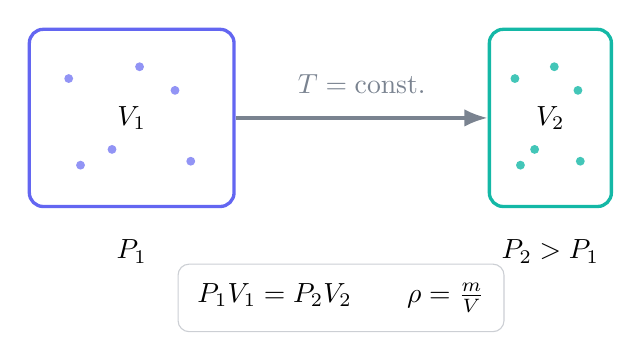
\begin{tikzpicture}[font=\sffamily,>=Latex]
  \node[draw=nebula,very thick,rounded corners=5pt,minimum width=2.6cm,minimum height=2.25cm] (v1) {$V_1$};
  \node[draw=spark,very thick,rounded corners=5pt,minimum width=1.55cm,minimum height=2.25cm,right=3.2cm of v1] (v2) {$V_2$};
  \draw[->,very thick,ink!65] (v1)--(v2) node[midway,above=5pt] {$T=\mathrm{const.}$};
  \foreach \x/\y in {-.8/.5,-.25/-.4,.55/.35,.75/-.55,-.65/-.6,.1/.65}{\fill[nebula!70] ($(v1)+(\x,\y)$) circle (1.6pt);}
  \foreach \x/\y in {-.45/.5,-.2/-.4,.35/.35,.38/-.55,-.38/-.6,.05/.65}{\fill[spark!80] ($(v2)+(\x,\y)$) circle (1.6pt);}
  \node[below=8pt of v1] {$P_1$};
  \node[below=8pt of v2] {$P_2>P_1$};
  \node[draw=ink!25,rounded corners=4pt,fill=white,inner sep=7pt,below=1.85cm of $(v1)!0.5!(v2)$]
    {$P_1V_1=P_2V_2\qquad \rho=\frac{m}{V}$};
\end{tikzpicture}
\end{document}
